%%%% CAPÍTULO 3 - MODELO COMPUTACIONAL E VERSÃO SEQUENCIAL

\chapter{Modelo computacional e versão sequencial}\label{cap:sequencial}

\section{Descrição do problema}

A população é representada por uma matriz de $L \times C$ células. Cada célula assume um dos estados:

\begin{itemize}
    \item \textbf{Ignorante (0)}: ainda não recebeu ou não acredita na informação;
    \item \textbf{Espalhador (1)}: acredita e compartilha a informação;
    \item \textbf{Inativo (2)}: recebeu a informação, mas não a compartilha mais.
\end{itemize}

\section{Regras de transição}

A cada geração, o novo estado de cada célula é calculado a partir da geração anterior:

\begin{itemize}
    \item um ignorante torna-se espalhador se possuir pelo menos $\lambda$ vizinhos espalhadores (limiar de convencimento);
    \item um espalhador torna-se inativo na geração seguinte;
    \item um inativo permanece inativo.
\end{itemize}

As bordas da matriz são fixas (sem continuidade toroidal): células da borda possuem menos de oito vizinhos. A grade inicial é gerada com semente fixa, e as regras de transição são determinísticas; portanto, para os mesmos parâmetros, a evolução é sempre a mesma. Essa propriedade é usada para verificar a correção das versões paralela e distribuída.

\section{Funcionamento da implementação sequencial}\label{sec:funcionamento-sequencial}

A implementação sequencial fornecida (\texttt{fakenews\_sequencial\_original.py}) é a referência de comportamento deste trabalho: as versões paralela e distribuída devem produzir, geração a geração, exatamente as mesmas grades que ela. O programa é um único arquivo em Python, organizado em cinco funções principais e uma função auxiliar de exibição, e segue o fluxo da Figura~\ref{fig:fluxograma-sequencial}.

\begin{figure}[!htb]
    \caption{Fluxograma da implementação sequencial}
    \label{fig:fluxograma-sequencial}
    \centering
    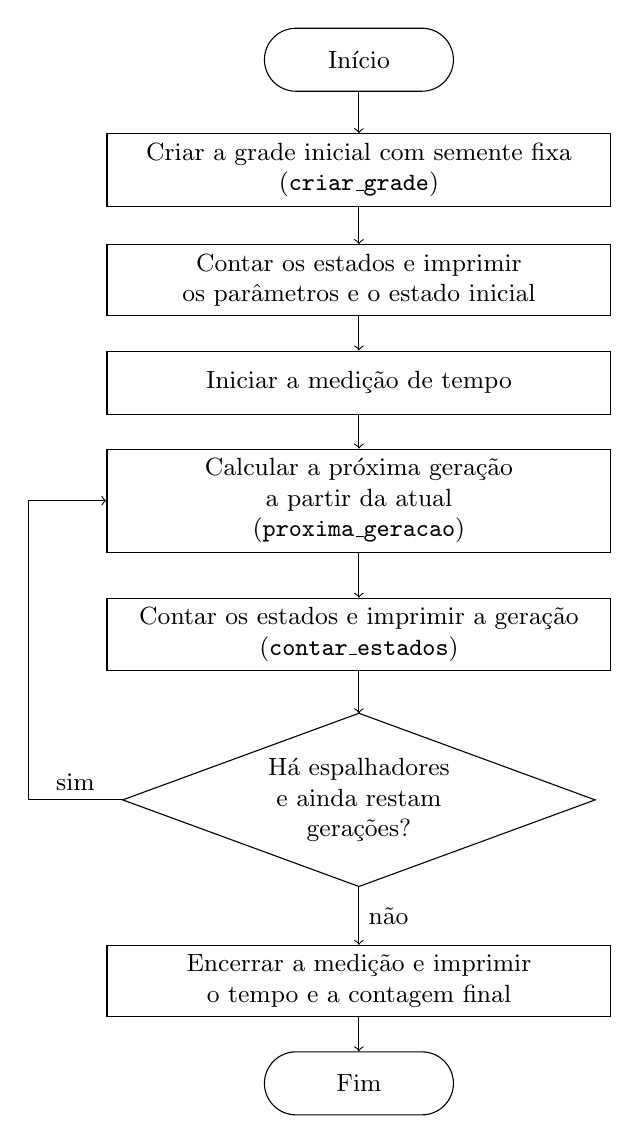
\begin{tikzpicture}[x=1cm, y=1cm, font=\small,
            etapa/.style={draw, align=center, minimum width=6.4cm, minimum height=0.8cm},
            extremo/.style={draw, rounded corners=0.4cm, minimum width=2.4cm, minimum height=0.8cm}]
        \node[extremo] (inicio) at (0, 0) {Início};
        \node[etapa] (criar) at (0, -1.4) {Criar a grade inicial com semente fixa\\(\texttt{criar\_grade})};
        \node[etapa] (inicial) at (0, -2.8) {Contar os estados e imprimir\\os parâmetros e o estado inicial};
        \node[etapa] (relogio) at (0, -4.1) {Iniciar a medição de tempo};
        \node[etapa] (proxima) at (0, -5.6) {Calcular a próxima geração\\a partir da atual\\(\texttt{proxima\_geracao})};
        \node[etapa] (contar) at (0, -7.3) {Contar os estados e imprimir a geração\\(\texttt{contar\_estados})};
        %% Losango desenhado com caminho próprio (sem biblioteca do TikZ)
        \draw (0, -8.3) -- (3.0, -9.4) -- (0, -10.5) -- (-3.0, -9.4) -- cycle;
        \node[align=center] at (0, -9.4) {Há espalhadores\\e ainda restam\\gerações?};
        \node[etapa] (final) at (0, -11.7) {Encerrar a medição e imprimir\\o tempo e a contagem final};
        \node[extremo] (fim) at (0, -13.0) {Fim};
        \draw[->] (inicio) -- (criar);
        \draw[->] (criar) -- (inicial);
        \draw[->] (inicial) -- (relogio);
        \draw[->] (relogio) -- (proxima);
        \draw[->] (proxima) -- (contar);
        \draw[->] (contar) -- (0, -8.3);
        \draw[->] (0, -10.5) -- node[right] {não} (final);
        \draw[->] (-3.0, -9.4) -- node[above] {sim} (-4.2, -9.4) |- (proxima.west);
        \draw[->] (final) -- (fim);
    \end{tikzpicture}
    \fonte{}
    \addcontentsline{loge}{figure}{\protect\numberline{\thefigure}Fluxograma da implementação sequencial}
\end{figure}

Primeiro, a grade inicial é criada e o estado inicial é impresso. Em seguida, cada iteração do laço calcula uma geração inteira e imprime a contagem dos estados. O laço termina quando não há mais espalhadores ou quando o número de gerações pedido é atingido; por fim, o programa imprime o tempo de execução e a distribuição final dos estados.

\subsection{Estrutura e funções}\label{sub:funcoes-sequencial}

A grade é uma lista de listas de inteiros, uma lista por linha, e os três estados são representados pelas constantes \texttt{IGNORANTE}~(0), \texttt{ESPALHADOR}~(1) e \texttt{INATIVO}~(2).

A função \texttt{criar\_grade} gera a população inicial. Ela inicializa o gerador pseudoaleatório do Python com \texttt{random.seed(semente)}, em que a semente vale 42 por padrão, preenche toda a grade com ignorantes e sorteia $\lfloor L \cdot C \cdot p \rfloor$ posições com \texttt{random.randint}, sendo $p$ o percentual inicial de espalhadores; cada posição sorteada torna-se espalhadora. O sorteio é feito com reposição: uma mesma célula pode ser sorteada mais de uma vez, e por isso o número real de espalhadores pode ser menor que o pedido. Na grade de $100 \times 100$ com 5\% de espalhadores, por exemplo, são feitos 500 sorteios, que resultam em 490 espalhadores; é por esse motivo que o programa imprime a quantidade de ``espalhadores reais''. Essa é a única parte aleatória do programa: como a semente é fixa, a mesma grade inicial é obtida em toda execução com os mesmos parâmetros.

A função \texttt{contar\_vizinhos\_espalhadores} recebe a grade e a posição $(i, j)$ de uma célula e conta quantos dos seus vizinhos na vizinhança de Moore são espalhadores. Para isso, percorre os deslocamentos $\Delta i, \Delta j \in \{-1, 0, 1\}$, descarta o par $(0, 0)$, que corresponde à própria célula, e só consulta a posição vizinha se ela estiver dentro da grade, isto é, se $0 \le i + \Delta i < L$ e $0 \le j + \Delta j < C$. É esse teste de limite que implementa as bordas fixas descritas na Seção~\ref{sec:automatos-celulares}: o vizinho que estaria fora da matriz simplesmente não é contado.

A função \texttt{proxima\_geracao} aplica as regras de transição a toda a grade. Ela cria a nova grade como uma cópia independente da atual (\texttt{deepcopy}) e percorre todas as células, linha a linha. Para cada célula ignorante, conta os vizinhos espalhadores e, se o total for maior ou igual ao limiar $\lambda$ (parâmetro \texttt{limiar\_convencimento}), marca a célula como espalhadora na nova grade; caso contrário, a célula mantém o valor copiado e continua ignorante. Cada espalhador passa a inativo, e cada inativo permanece inativo. A contagem de vizinhos é feita apenas para as células ignorantes, pois só elas mudam de estado por influência dos vizinhos. Durante toda a varredura, os estados são lidos somente da grade atual e escritos somente na nova grade; assim, nenhuma célula enxerga o estado já atualizado de um vizinho, o que implementa a atualização síncrona apresentada na Seção~\ref{sec:automatos-celulares}. Ao final, a nova grade é devolvida e passa a ser a grade atual.

A função \texttt{contar\_estados} percorre a grade inteira e devolve um dicionário com a quantidade de células em cada estado. Esses totais são usados tanto para imprimir o andamento da simulação quanto para decidir a parada. A função auxiliar \texttt{imprimir\_grade} mostra no terminal até $30 \times 30$ células da grade, com os símbolos ``.'', ``E'' e ``N'', e só é chamada quando a opção \texttt{mostrar\_grade} está ativada.

Por fim, a função \texttt{executar\_simulacao} coordena a execução descrita na Figura~\ref{fig:fluxograma-sequencial}. Seus parâmetros são o número de linhas e de colunas, o número máximo de gerações, o percentual inicial de espalhadores, o limiar de convencimento e a opção \texttt{mostrar\_grade}. Os valores padrão da função são uma grade de $100 \times 100$, 50~gerações, 2\% de espalhadores e limiar~2, mas o bloco principal do arquivo a chama com 5\% de espalhadores e limiar~3. Depois de criar a grade e imprimir os parâmetros e a contagem inicial, a função executa o laço de gerações; após cada geração, imprime uma linha com as quantidades de ignorantes, espalhadores e inativos e interrompe o laço antecipadamente se não houver mais espalhadores, já que, sem eles, nenhum ignorante pode ser convencido e a grade não muda mais. O tempo de execução é medido com \texttt{time.time()} imediatamente antes e depois do laço, de modo que o intervalo medido inclui o cálculo, a contagem e as impressões de cada geração. Ao final, são impressos esse tempo e a quantidade e o percentual de células em cada estado.

\subsection{Exemplo de execução}\label{sub:exemplo-sequencial}

Para ilustrar o funcionamento passo a passo, a Figura~\ref{fig:exemplo-sequencial} mostra a evolução de uma grade de $5 \times 5$ criada pela própria função \texttt{criar\_grade}, com semente~42 e 12\% de espalhadores (três sorteios, que resultaram em três espalhadores), e evoluída por \texttt{proxima\_geracao} com limiar $\lambda = 2$. As posições são indicadas por (linha, coluna), numeradas a partir de 0, como no código. Abaixo de cada grade aparecem as quantidades de ignorantes (I), espalhadores (E) e inativos (N), as mesmas que o programa imprime a cada geração.

\begin{figure}[!htb]
    \caption{Exemplo de evolução de uma grade de 5~$\times$~5 com limiar 2}
    \label{fig:exemplo-sequencial}
    \centering
    %% Gerado executando criar_grade(5, 5, 0.12) e proxima_geracao(grade, 2) do código fornecido.
    %% \painel{x}{y}{espalhadores}{inativos}{geração}{contagem}; posições em linha/coluna.
    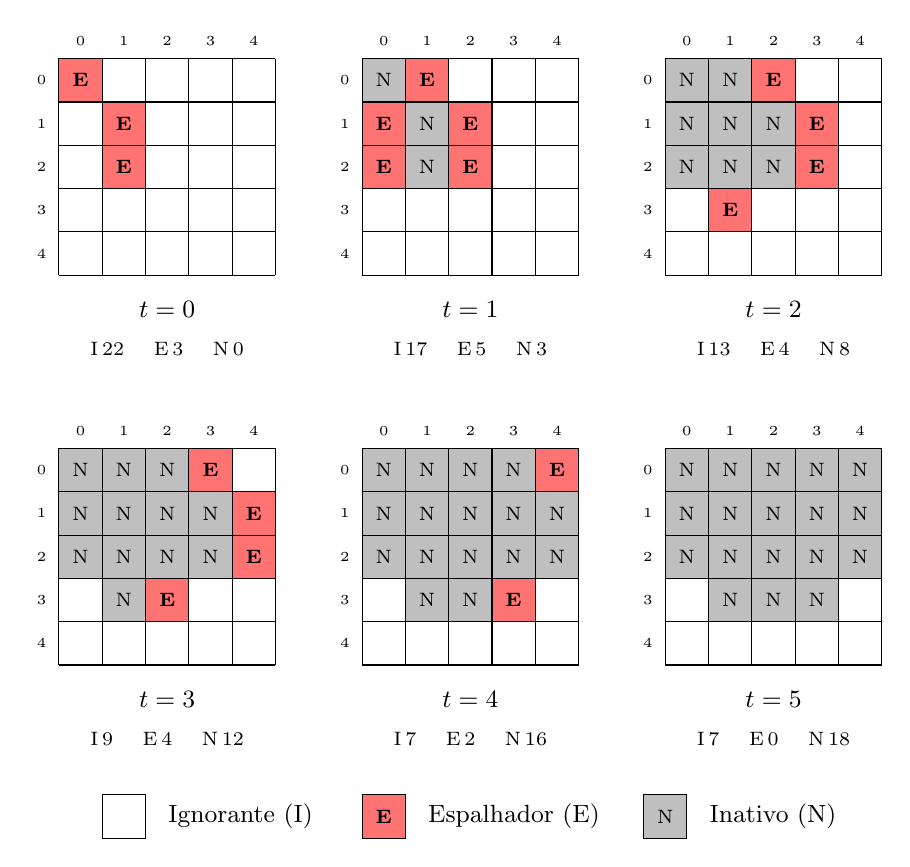
\begin{tikzpicture}[x=0.55cm, y=0.55cm]
        \newcommand*{\painel}[6]{%
            \begin{scope}[shift={(#1,#2)}]
                \foreach \i/\j in {#3} {\filldraw[fill=red!55] (\j,-\i) rectangle +(1,-1) node[midway] {\scriptsize\textbf{E}};}
                \foreach \i/\j in {#4} {\filldraw[fill=black!25] (\j,-\i) rectangle +(1,-1) node[midway] {\scriptsize N};}
                \foreach \k in {0,...,5} {\draw (\k,0) -- (\k,-5); \draw (0,-\k) -- (5,-\k);}
                \foreach \k in {0,...,4} {
                    \node[font=\tiny] at (\k+0.5, 0.4) {\k};
                    \node[font=\tiny] at (-0.4, -\k-0.5) {\k};
                }
                \node[font=\small] at (2.5,-5.8) {#5};
                \node[font=\scriptsize] at (2.5,-6.7) {#6};
            \end{scope}}
        \painel{0}{0}{0/0,1/1,2/1}{}{$t=0$}{I\,22 \quad E\,3 \quad N\,0}
        \painel{7}{0}{0/1,1/0,1/2,2/0,2/2}{0/0,1/1,2/1}{$t=1$}{I\,17 \quad E\,5 \quad N\,3}
        \painel{14}{0}{0/2,1/3,2/3,3/1}{0/0,0/1,1/0,1/1,1/2,2/0,2/1,2/2}{$t=2$}{I\,13 \quad E\,4 \quad N\,8}
        \painel{0}{-9}{0/3,1/4,2/4,3/2}{0/0,0/1,0/2,1/0,1/1,1/2,1/3,2/0,2/1,2/2,2/3,3/1}{$t=3$}{I\,9 \quad E\,4 \quad N\,12}
        \painel{7}{-9}{0/4,3/3}{0/0,0/1,0/2,0/3,1/0,1/1,1/2,1/3,1/4,2/0,2/1,2/2,2/3,2/4,3/1,3/2}{$t=4$}{I\,7 \quad E\,2 \quad N\,16}
        \painel{14}{-9}{}{0/0,0/1,0/2,0/3,0/4,1/0,1/1,1/2,1/3,1/4,2/0,2/1,2/2,2/3,2/4,3/1,3/2,3/3}{$t=5$}{I\,7 \quad E\,0 \quad N\,18}
        %% Legenda
        \draw (1,-17) rectangle +(1,-1);
        \node[anchor=west, font=\small] at (2.3,-17.5) {Ignorante (I)};
        \filldraw[fill=red!55] (7,-17) rectangle +(1,-1) node[midway] {\scriptsize\textbf{E}};
        \node[anchor=west, font=\small] at (8.3,-17.5) {Espalhador (E)};
        \filldraw[fill=black!25] (13.5,-17) rectangle +(1,-1) node[midway] {\scriptsize N};
        \node[anchor=west, font=\small] at (14.8,-17.5) {Inativo (N)};
    \end{tikzpicture}
    \fonte{}
    \addcontentsline{loge}{figure}{\protect\numberline{\thefigure}Exemplo de evolução de uma grade de 5~$\times$~5 com limiar 2}
\end{figure}

Na geração inicial ($t=0$), há espalhadores em (0,0), (1,1) e (2,1). A célula (1,0), na borda esquerda, tem apenas cinco vizinhos, mas três deles são espalhadores; as células (0,1), (1,2), (2,0) e (2,2) têm dois vizinhos espalhadores cada. Todas atingem o limiar e tornam-se espalhadoras em $t=1$. Já as células (0,2), (3,0), (3,1) e (3,2) têm apenas um vizinho espalhador e continuam ignorantes. Os três espalhadores iniciais tornam-se inativos: cada espalhador propaga a notícia durante uma única geração.

Em $t=1$, os cinco novos espalhadores formam uma frente em volta das células que se tornaram inativas. Convertem-se as células (0,2), (1,3) e (2,3), com dois vizinhos espalhadores cada, e (3,1), cujos vizinhos espalhadores são (2,0) e (2,2). A célula (2,1) também é vizinha de (3,1), mas, por estar inativa, não é contada: inativos não influenciam ninguém. A célula (3,0) tem novamente apenas um vizinho espalhador, (2,0), e continua ignorante.

Em $t=2$, a frente continua a avançar para a direita e para baixo. Tornam-se espalhadoras (0,3), (1,4) e (2,4), e também (3,2), cujos vizinhos espalhadores são (2,3) e (3,1). As demais células ignorantes têm no máximo um vizinho espalhador e não mudam; entre elas estão (3,0) e as células (4,0), (4,1) e (4,2) da última linha, vizinhas apenas de (3,1).

Em $t=3$, somente duas células atingem o limiar: (0,4), no canto superior direito, vizinha de (0,3) e (1,4), e (3,3), vizinha de (2,4) e (3,2). As outras células ignorantes, como (3,4) e as da última linha, têm no máximo um vizinho espalhador, e a frente começa a se desfazer.

Em $t=4$, os dois espalhadores restantes estão isolados: (0,4) só tem vizinhos inativos, e cada célula ignorante vizinha de (3,3), isto é, (3,4), (4,2), (4,3) e (4,4), tem apenas esse vizinho espalhador. Nenhuma célula é convertida, e em $t=5$ não há mais espalhadores. Nesse ponto, \texttt{executar\_simulacao} interrompe o laço, mesmo que o número de gerações pedido seja maior, e a grade termina com 7 ignorantes e 18 inativos: as células (3,0) e (3,4) e toda a última linha nunca tiveram dois vizinhos espalhadores na mesma geração.

O exemplo evidencia dois aspectos que determinam a dinâmica do modelo. Como cada espalhador atua por uma única geração, as influências recebidas em gerações diferentes não se acumulam: uma célula só é convertida se tiver ao menos $\lambda$ vizinhos espalhadores ao mesmo tempo. Por isso, quando a frente de propagação se estreita, por exemplo junto às bordas, onde há menos vizinhos, ela deixa de atingir o limiar, e a propagação se extingue antes de alcançar toda a população.

\subsection{Versão sequencial refatorada}\label{sub:sequencial-refatorada}

Além do código fornecido, foi desenvolvida uma versão sequencial refatorada (\texttt{sequencial/fakenews\_sequencial.py}), que usa o mesmo núcleo de cálculo das versões paralela e distribuída (\texttt{comum/modelo.py}). Ela mantém as regras de transição e a grade inicial, gerada pela própria função \texttt{criar\_grade} com a mesma semente, e muda apenas a representação dos dados: a grade passa a ser um vetor de bytes com uma linha de zeros acima e outra abaixo, e duas grades são alternadas entre as gerações, em vez de uma cópia com \texttt{deepcopy} a cada geração. Testes automatizados verificam que ela produz, geração a geração, as mesmas grades que o código original. Essa versão é a linha de base dos experimentos (Seção~\ref{cap:experimentos}), pois executa o mesmo cálculo das versões paralela e distribuída sem nenhum custo de comunicação ou de sincronização; seus detalhes são apresentados na Seção~\ref{cap:melhorias}. A seguir, analisa-se o custo computacional da implementação sequencial.

\section{Análise de custo}\label{sec:custo-sequencial}

Esta seção analisa o custo de tempo e de memória da implementação fornecida. Primeiro, o custo é estimado a partir do código; em seguida, a estimativa é comparada com medições, e discute-se como os parâmetros do modelo afetam a duração da simulação. As medições foram feitas com os \textit{scripts} da pasta \texttt{experimentos/} do repositório, sempre com a grade inicial de semente~42.

\subsection{Custo por geração}\label{sub:custo-geracao}

Em cada geração, \texttt{proxima\_geracao} copia a grade com \texttt{deepcopy} e visita uma vez cada uma das $L \cdot C$ células. O trabalho por célula depende do estado: uma célula ignorante chama \texttt{contar\_vizinhos\_espalhadores}, que percorre os nove deslocamentos da vizinhança, descarta o central e testa se cada vizinho está dentro da grade antes de consultá-lo, enquanto um espalhador ou um inativo exige apenas a comparação do estado e uma atribuição. Em seguida, \texttt{contar\_estados} percorre a grade inteira mais uma vez. Sendo $N_I$ o número de células ignorantes na geração, o tempo de uma geração pode ser escrito como
\begin{equation}\label{eq:custo-geracao}
    T_{\mathrm{ger}} \approx c_I \, N_I + c_O \, (L C - N_I) + (c_{\mathrm{cop}} + c_{\mathrm{cont}}) \, L C ,
\end{equation}
em que $c_I$ e $c_O$ são os custos de visitar uma célula ignorante e uma célula de outro estado, e $c_{\mathrm{cop}}$ e $c_{\mathrm{cont}}$ são os custos por célula da cópia e da contagem. Todos os termos são proporcionais ao tamanho da grade; logo, uma geração custa $\Theta(L \cdot C)$, e a simulação inteira custa $\Theta(G_{\mathrm{ef}} \cdot L \cdot C)$, em que $G_{\mathrm{ef}} \le G$ é o número de gerações efetivamente executadas, que pode ser menor que o pedido por causa da parada antecipada.

A memória também cresce com $L \cdot C$. A grade é uma lista de listas de inteiros; no CPython, cada posição de uma lista guarda uma referência de 8~bytes para um objeto inteiro, e os inteiros pequenos, como 0, 1 e 2, são objetos compartilhados. Por isso, a grade ocupa cerca de 8,9~bytes por célula, quase todos gastos com referências: 8,45~MiB para uma grade de $1000 \times 1000$, medidos com o módulo \texttt{tracemalloc}. Durante \texttt{proxima\_geracao}, a grade atual e a cópia existem ao mesmo tempo, e a memória ocupada dobra, chegando a cerca de 17~MiB nessa grade. Para comparação, a mesma grade guardada como vetor de bytes, como na versão refatorada, ocupa cerca de 1~byte por célula.

\subsection{Medições}\label{sub:custo-medicoes}

Para verificar a estimativa, a Tabela~\ref{tab:custo-escala} mostra o tempo do laço de gerações do código fornecido em três tamanhos de grade, com 20~gerações, 5\% de espalhadores e limiar~2, sem impressão no terminal. As medições foram feitas em um processador Intel Core i9-12900F, com Windows~11 e Python~3.11.7, e o valor apresentado é a mediana de três repetições.

\begin{table}[htb]
    \centering
    \caption{Tempo do laço de gerações do código fornecido conforme o tamanho da grade}
    \label{tab:custo-escala}
    \begin{tabular}{lrrrr}
        \toprule
        \textbf{Grade} & \textbf{Células} & \textbf{Tempo (s)} & \textbf{Por geração (s)} & \textbf{Por célula e geração ($\mu$s)} \\
        \midrule
        $500 \times 500$   & 250\,000     & 4,16  & 0,208 & 0,83 \\
        $1000 \times 1000$ & 1\,000\,000  & 16,46 & 0,823 & 0,82 \\
        $2000 \times 2000$ & 4\,000\,000  & 65,88 & 3,294 & 0,82 \\
        \bottomrule
    \end{tabular}
    \fonte{}
\end{table}

Quando o número de células é multiplicado por quatro, o tempo também é multiplicado por quatro, e o tempo por célula e por geração permanece em torno de 0,82~$\mu$s: o custo cresce linearmente com $L \cdot C$, como previsto. Esse valor corresponde a milhares de ciclos de relógio do processador por célula, o que reflete o custo de interpretar o código Python, em que cada acesso a uma lista, comparação ou chamada de função é executado pelo interpretador.

A Tabela~\ref{tab:custo-perfil} mostra como o tempo de uma geração se divide entre as etapas. Essa medição foi feita em outra máquina (Intel Core i7-13650HX, Windows~11, Python~3.12.10), na grade de $1000 \times 1000$ e com os mesmos parâmetros, e o valor apresentado é a mediana de cinco repetições, após uma execução de aquecimento descartada. Como o \texttt{deepcopy} ocorre dentro de \texttt{proxima\_geracao} e o código fornecido não foi alterado, a cópia foi medida à parte, sobre uma cópia da mesma grade, e o tempo da varredura foi obtido por diferença; os valores dessas duas linhas são, portanto, estimativas.

\begin{table}[htb]
    \centering
    \caption{Divisão do tempo de uma geração do código fornecido}
    \label{tab:custo-perfil}
    \begin{tabular}{lrr}
        \toprule
        \textbf{Etapa} & \textbf{Por geração (s)} & \textbf{Participação (\%)} \\
        \midrule
        Varredura das células                           & 0,638 & 74,6 \\
        Cópia da grade (\texttt{deepcopy})              & 0,179 & 21,0 \\
        Contagem dos estados (\texttt{contar\_estados}) & 0,038 & 4,4 \\
        \midrule
        Total                                          & 0,855 & 100,0 \\
        \bottomrule
    \end{tabular}
    \fonte{}
\end{table}

A varredura das células responde por cerca de três quartos do tempo, e a cópia, por cerca de um quinto. A cópia não contribui para o cálculo: ela pode ser evitada alternando duas grades entre as gerações, como faz a versão refatorada, cujo ganho é apresentado na Seção~\ref{cap:melhorias}.

O perfil também confirma que o custo depende do estado das células. Ao longo das 20~gerações, o número de ignorantes cai de cerca de 951~mil para 440~mil, e o tempo da varredura cai junto, com correlação de 0,999. Ajustando uma reta pelo método dos mínimos quadrados ao tempo da varredura em função do número de ignorantes, conforme a Equação~\ref{eq:custo-geracao}, obtêm-se $c_I \approx 1,02$~$\mu$s por célula ignorante e $c_O \approx 0,06$~$\mu$s por célula nos demais estados. Como $c_O$ vem do prolongamento da reta até $N_I = 0$, fora da faixa medida, seu valor é menos preciso que o de $c_I$; ainda assim, visitar um ignorante custa mais de dez vezes o que custa visitar uma célula de outro estado. Essa diferença faz com que regiões da grade com mais ignorantes demorem mais para ser calculadas, o que é a origem do desbalanceamento de carga discutido nas versões paralela e distribuída.

\subsection{Influência dos parâmetros}\label{sub:custo-parametros}

Como o custo total é $\Theta(G_{\mathrm{ef}} \cdot L \cdot C)$, o número de gerações efetivamente executadas também pesa, e ele depende fortemente do limiar e do percentual inicial de espalhadores. A Tabela~\ref{tab:custo-limiar} mostra, para a grade de $1000 \times 1000$, quantas gerações a simulação dura até não haver mais espalhadores e qual fração da população deixou de ser ignorante (alcance); em cada célula da tabela, o primeiro número é a quantidade de gerações e o valor entre parênteses é o alcance. Esses valores não dependem da máquina e foram obtidos com a versão refatorada, que produz as mesmas grades que o código fornecido.

\begin{table}[htb]
    \centering
    \caption{Gerações até a propagação terminar e alcance final, conforme o limiar e o percentual inicial de espalhadores}
    \label{tab:custo-limiar}
    \begin{tabular}{lrrrr}
        \toprule
        \textbf{Limiar} & \textbf{1\%} & \textbf{2\%} & \textbf{5\%} & \textbf{10\%} \\
        \midrule
        $\lambda = 1$ & 27 (100,0\%) & 15 (100,0\%) & 10 (100,0\%) & 7 (100,0\%) \\
        $\lambda = 2$ & 264 (14,3\%) & 163 (25,2\%) & 56 (57,9\%) & 29 (90,8\%) \\
        $\lambda = 3$ & 2 (1,0\%) & 3 (2,0\%) & 3 (5,4\%) & 4 (12,8\%) \\
        \bottomrule
    \end{tabular}
    \fonte{}
\end{table}

Com $\lambda = 1$, um único vizinho espalhador basta, e a notícia alcança toda a população em poucas gerações. Com $\lambda = 3$, é raro uma célula ter três vizinhos espalhadores ao mesmo tempo, e a propagação termina em até quatro gerações, alcançando pouco mais que os espalhadores iniciais. Com $\lambda = 2$, a simulação é a mais longa, chegando a 264~gerações com 1\% de espalhadores, e o alcance varia de 14\% a 91\% conforme o percentual inicial. Por isso, os parâmetros usados no bloco principal do código fornecido ($\lambda = 3$ e 5\%) encerram a simulação em três gerações e não servem para medir desempenho. Nos experimentos (Seção~\ref{cap:experimentos}), foram usados $\lambda = 2$ e 5\% de espalhadores com 20~gerações: como, nesse cenário, a propagação dura 56~gerações, todas as execuções completam as 20~gerações, e o trabalho medido é o mesmo em todas as versões.

\subsection{Potencial de paralelização}\label{sub:custo-paralelizacao}

A análise também indica o que pode ser paralelizado. O novo estado de cada célula depende apenas da geração anterior; portanto, as $L \cdot C$ atualizações de uma geração são independentes entre si e podem ser divididas entre vários trabalhadores, sem comunicação durante o cálculo. A contagem dos estados também pode ser feita por partes e somada ao final. A dependência existe apenas entre gerações: a geração $t+1$ só pode começar quando a geração $t$ estiver completa, e a decisão de parada exige a soma das contagens de toda a grade. Essas duas restrições definem os pontos de sincronização das versões paralela e distribuída, apresentadas nas seções~\ref{cap:paralela} e~\ref{cap:distribuida}.
